\label{sec:4.3}

%%%%%%%%%%%%%%%%%%%%%%%%%%%%%%%%%%%%%%%%%%%%%%%%%%%%%%%
% Dynamic Linearity
%%%%%%%%%%%%%%%%%%%%%%%%%%%%%%%%%%%%%%%%%%%%%%%%%%%%%%%

The dynamic performance of an ADC is determined by the effective number of bits (ENOB). Figure~\ref{fig:coldadc_fft} shows the Fast-Fourier Transform (FFT) from one of the ADC channels.  The ENOB across ADC channels at LN$_2$ temperature is generally fairly uniform with a mean value of 10.6 and an RMS of about 0.3 bits. Table~\ref{tab:adc_enob} lists the measured ENOB for the 16 ADC channels from one of the ASICs tested.
\begin{figure}[htb]
\centering
%\begin{minipage}[b]{1.0\textwidth}
\begin{center}
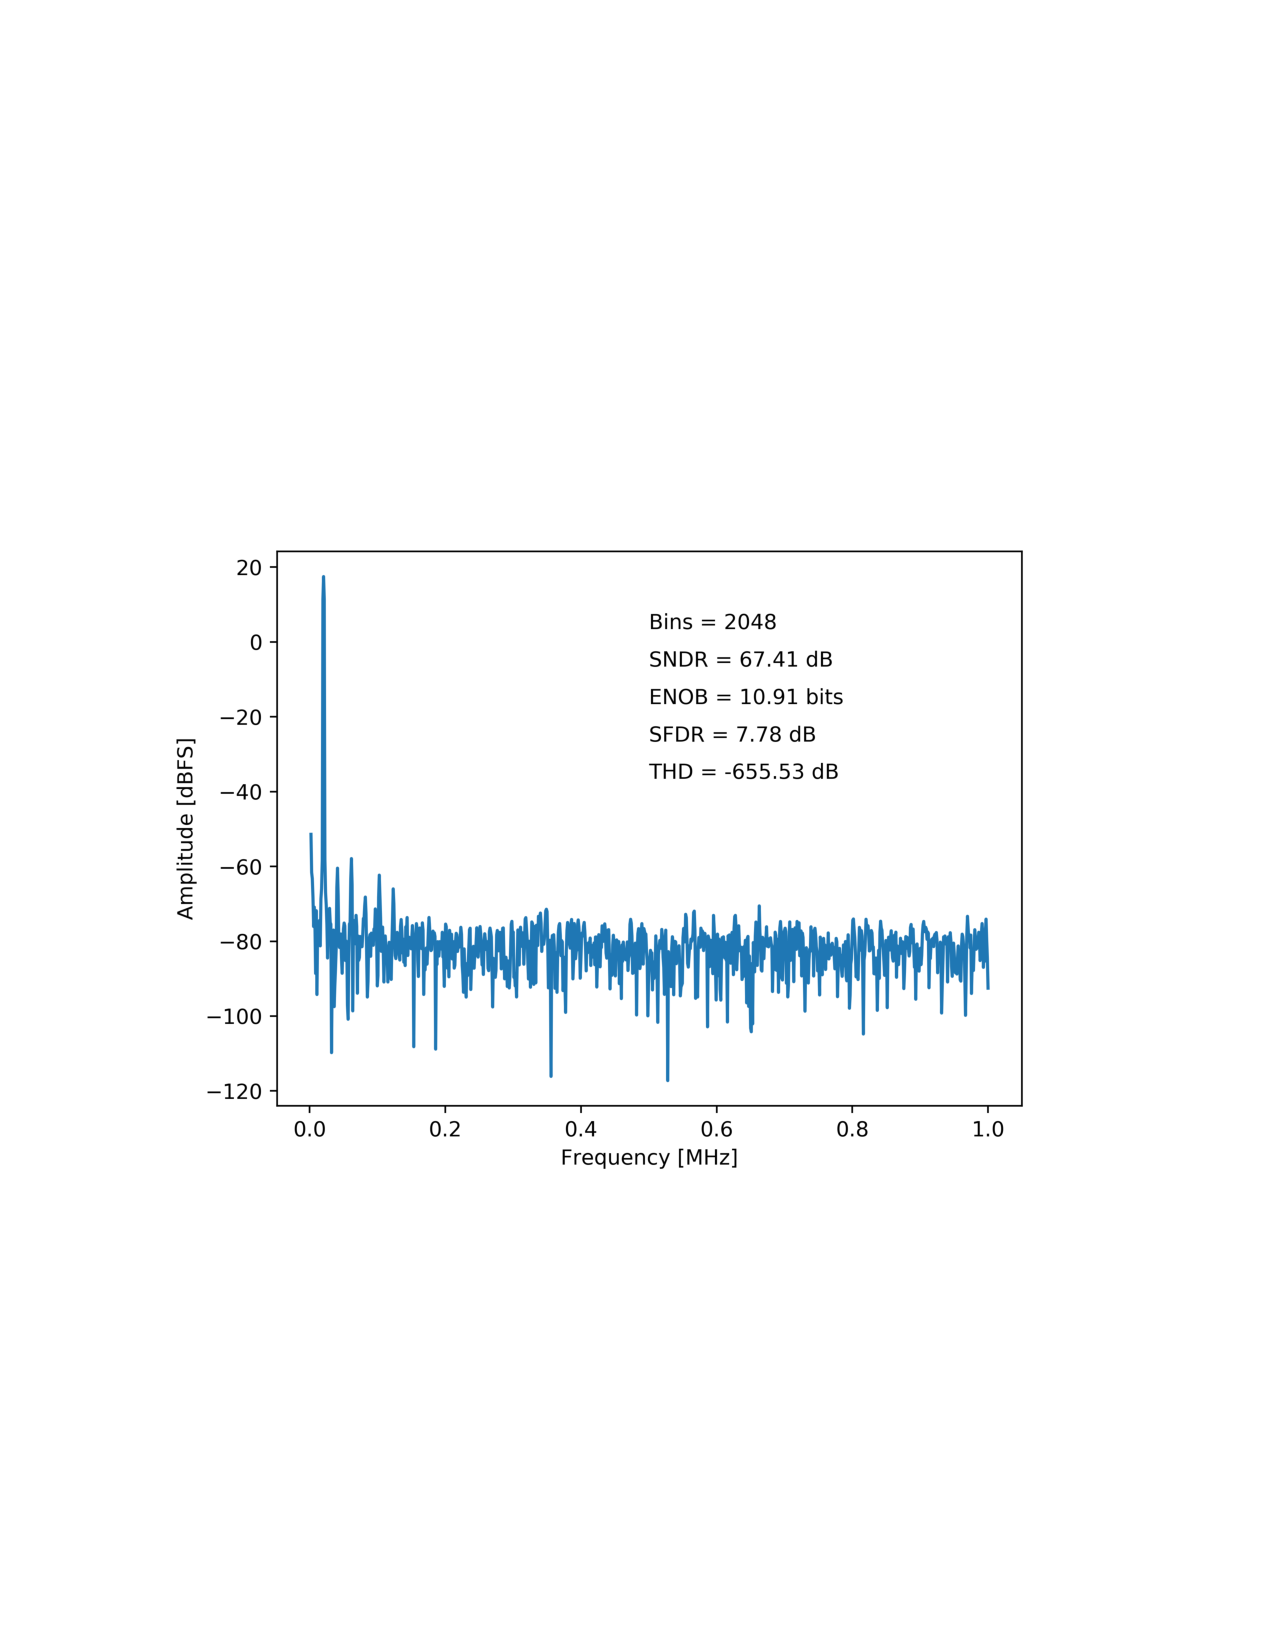
\includegraphics[width=0.7\textwidth]{figures/fft_Sinusoid_20KHz_SE-SHA-ADC0_NomVREFPN_2M_v1.pdf}
\end{center}
%\end{minipage}
\caption{FFT.}
\label{fig:coldadc_fft}
\end{figure}

\begin{table}[h]
\centering
\begin{tabular}{|c|c|c|c|c|c|c|c|c|}
\hline
\textbf{ Channel\# } & Ch0&Ch1&Ch2&Ch3 &Ch4 &Ch5 &Ch6 &Ch7 \\ \hline 
\textbf{ ENOB } & 10.5 & 10.8 & 10.2 & 10.4 & 10.7 & 9.8 & 10.6 & 10.4\\ \hline \hline
\textbf{ Channel\# } & Ch8&Ch9&Ch10&Ch11 &Ch12 &Ch13 &Ch14 &Ch15 \\ \hline
\textbf{ ENOB } & 10.2 & 10.5  & 10.6 & 10.5 & 10.7 & 10.3 & 9.8 & 9.7 \\ \hline
\end{tabular}
\caption{ColdADC ASIC\# ENOB vs channel in LN$_2$.}
\label{tab:adc_enob}
\end{table}


